\section{Оптимизация геометрических параметров сечения центроплана}
\subsection{Постановка задачи}
В ходе работы было проведено исследование зависимости веса центроплана от его параметров с учетом критерия неразрушения конструкции при заданных нагрузках. Для этого была решена следующая модельная задача.

\subsection{Постановка модельной задачи}
Имеется упрощенная модель центроплана -- короб переменного прямоугольного сечения с перегородками. На него передаются нагрузки посредством приложения аэродинамических нагрузок на модель крыла -- короб постоянного прямоугольного сечения. Для модели центроплана имеются два параметра: относительная координата нижней точки сечения и строительная высота в плоскости симметрии самолета. Было выбрано 42 пары параметров, для каждой пары проведена оптимизация сечения с целью удовлетворения требований прочности конструкции, а именно: среднее напряжение в каждой панели не должно превышать допускаемого напряжения, равного $35\text{кг}/\text{мм}^2$. Оптимизация проводилась алгоритмом $\sigma/\sigma$ для каждой панели. Итоговые результаты вычислений приведены в таблице \ref{tab:KessOptimBigTable} и на Рис.\ref{fig:Optimization3dplot}

\tabulinesep = 1mm
\definecolor{lightgray}{gray}{0.9}
\begin{table}[H]
\captionsetup{justification=centering}
\caption{Зависимость площади панелей центроплана и веса кессона от параметров центроплана}
%\rowcolors{2}{}{lightgray}
\begin{tabu}to \linewidth{|c|*4{X[m c]|}*4{X[m c]|}}
\hline
\multirow{2}{*}[-1.1ex]{N} & \multicolumn{4}{c|}{Вес кессона~[кг]} & \multicolumn{4}{c|}{Площадь панелей центроплана~[$\text{м}^2$]} \\ \cline{2-9}
& Верхние панели & Нижние панели & Боковые стенки & $\Sigma$ & Верхние панели & Нижние панели & Боковые стенки & $\Sigma$ \\
\hline
\taburowcolors {lightgray .. white}
1 & 297.182 & 294.551 & 12.561 & 604.294 & 2.730 & 2.730 & 4.000 & 9.520\\ \hline
2 & 225.261 & 237.378 & 27.672 & 490.313 & 2.730 & 2.740 & 5.210 & 10.720\\ \hline
3 & 190.080 & 222.327 & 49.159 & 461.564 & 2.730 & 2.760 & 5.820 & 11.340\\ \hline
4 & 161.544 & 211.467 & 65.963 & 438.972 & 2.730 & 2.760 & 6.450 & 11.950\\ \hline
5 & 146.581 & 199.989 & 66.844 & 413.415 & 2.730 & 2.780 & 7.090 & 12.590\\ \hline
6 & 134.746 & 191.293 & 70.912 & 396.952 & 2.730 & 2.800 & 7.640 & 13.200\\ \hline
7 & 350.816 & 374.021 & 47.679 & 772.515 & 2.910 & 2.910 & 4.000 & 9.850\\ \hline
8 & 253.752 & 259.311 & 53.180 & 566.245 & 2.910 & 2.850 & 5.210 & 10.990\\ \hline
9 & 213.881 & 226.655 & 57.618 & 498.154 & 2.910 & 2.830 & 5.840 & 11.570\\ \hline
10 & 188.442 & 205.603 & 62.047 & 456.092 & 2.910 & 2.810 & 6.450 & 12.150\\ \hline
11 & 174.466 & 196.192 & 66.506 & 437.164 & 2.910 & 2.780 & 7.090 & 12.770\\ \hline
12 & 154.328 & 195.919 & 70.963 & 421.210 & 2.910 & 2.770 & 7.680 & 13.350\\ \hline
13 & 363.681 & 391.414 & 48.862 & 803.953 & 3.010 & 3.000 & 4.000 & 10.000\\ \hline
14 & 258.118 & 275.555 & 53.209 & 586.883 & 3.010 & 2.930 & 5.230 & 11.160\\ \hline
15 & 225.322 & 238.220 & 57.604 & 521.145 & 3.010 & 2.890 & 5.820 & 11.720\\ \hline
16 & 201.612 & 214.755 & 62.046 & 478.413 & 3.010 & 2.860 & 6.440 & 12.310\\ \hline
17 & 171.877 & 203.370 & 66.418 & 441.665 & 3.010 & 2.840 & 7.050 & 12.900\\ \hline
18 & 163.553 & 201.207 & 70.912 & 435.673 & 3.010 & 2.820 & 7.660 & 13.480\\ \hline
19 & 380.079 & 398.521 & 49.032 & 827.631 & 3.050 & 3.050 & 4.000 & 10.110\\ \hline
20 & 267.143 & 279.590 & 53.134 & 599.866 & 3.050 & 2.980 & 5.210 & 11.240\\ \hline
21 & 231.158 & 238.954 & 57.667 & 527.779 & 3.050 & 2.930 & 5.820 & 11.820\\ \hline
22 & 197.327 & 218.001 & 62.040 & 477.368 & 3.050 & 2.910 & 6.410 & 12.390\\ \hline
23 & 191.553 & 205.935 & 66.481 & 463.971 & 3.050 & 2.870 & 7.070 & 12.980\\ \hline
24 & 158.352 & 203.948 & 70.897 & 433.199 & 3.050 & 2.850 & 7.660 & 13.560\\ \hline
25 & 383.525 & 410.374 & 50.351 & 844.249 & 3.110 & 3.110 & 4.000 & 10.210\\ \hline
26 & 279.228 & 288.331 & 53.186 & 620.745 & 3.110 & 3.030 & 5.210 & 11.350\\ \hline
27 & 233.614 & 249.500 & 57.583 & 540.696 & 3.110 & 2.990 & 5.820 & 11.910\\ \hline
28 & 213.922 & 221.683 & 62.125 & 497.728 & 3.110 & 2.950 & 6.450 & 12.500\\ \hline
29 & 180.457 & 210.067 & 66.523 & 457.046 & 3.110 & 2.920 & 7.070 & 13.070\\ \hline
30 & 167.492 & 205.426 & 71.001 & 443.918 & 3.110 & 2.880 & 7.640 & 13.660\\ \hline
31 & 401.418 & 424.040 & 50.413 & 875.868 & 3.160 & 3.160 & 4.000 & 10.330\\ \hline
32 & 285.115 & 297.451 & 53.649 & 636.214 & 3.160 & 3.070 & 5.230 & 11.470\\ \hline
33 & 251.131 & 255.015 & 57.656 & 563.801 & 3.160 & 3.040 & 5.860 & 12.030\\ \hline
34 & 212.049 & 229.543 & 62.067 & 503.658 & 3.160 & 3.000 & 6.450 & 12.610\\ \hline
35 & 191.030 & 215.968 & 66.550 & 473.548 & 3.160 & 2.970 & 7.070 & 13.170\\ \hline
36 & 170.765 & 209.184 & 70.962 & 450.912 & 3.160 & 2.920 & 7.660 & 13.740\\ \hline
37 & 431.880 & 451.562 & 51.974 & 935.418 & 3.230 & 3.230 & 4.000 & 10.440\\ \hline
38 & 291.199 & 306.178 & 54.263 & 651.640 & 3.230 & 3.130 & 5.210 & 11.560\\ \hline
39 & 253.054 & 265.073 & 57.593 & 575.719 & 3.230 & 3.090 & 5.820 & 12.140\\ \hline
40 & 222.782 & 233.403 & 61.948 & 518.132 & 3.230 & 3.050 & 6.400 & 12.700\\ \hline
41 & 197.192 & 218.301 & 66.423 & 481.917 & 3.230 & 3.020 & 7.030 & 13.270\\ \hline
42 & 175.591 & 210.828 & 70.877 & 457.295 & 3.230 & 2.970 & 7.660 & 13.840\\ \hline

\end{tabu}

\label{tab:KessOptimBigTable}
\end{table}


\tabulinesep = 1mm
\definecolor{lightgray}{gray}{0.9}
\begin{table}[H]
\captionsetup{justification=centering}
\caption{Зависимость площади панелей центроплана и веса кессона от параметров центроплана относительно варианта с прямым кессоном}
%\rowcolors{2}{}{lightgray}
\begin{tabu}to \linewidth{|c|*4{X[m c]|}*4{X[m c]|}}
\hline
\multirow{2}{*}[-1.1ex]{N} & \multicolumn{4}{c|}{Вес кессона} & \multicolumn{4}{c|}{Площадь панелей центроплана} \\ \cline{2-9}
& Верхние панели & Нижние панели & Боковые стенки & $\Sigma$ & Верхние панели & Нижние панели & Боковые стенки & $\Sigma$ \\
\hline
\taburowcolors {lightgray .. white}
1 & 0.492 & 0.487 & 0.021 & 1.000 & 0.287 & 0.287 & 0.420 & 1.000\\ \hline
2 & 0.373 & 0.393 & 0.046 & 0.811 & 0.287 & 0.288 & 0.547 & 1.126\\ \hline
3 & 0.315 & 0.368 & 0.081 & 0.764 & 0.287 & 0.290 & 0.611 & 1.191\\ \hline
4 & 0.267 & 0.350 & 0.109 & 0.726 & 0.287 & 0.290 & 0.678 & 1.255\\ \hline
5 & 0.243 & 0.331 & 0.111 & 0.684 & 0.287 & 0.292 & 0.745 & 1.322\\ \hline
6 & 0.223 & 0.317 & 0.117 & 0.657 & 0.287 & 0.294 & 0.803 & 1.387\\ \hline
7 & 0.581 & 0.619 & 0.079 & 1.278 & 0.306 & 0.306 & 0.420 & 1.035\\ \hline
8 & 0.420 & 0.429 & 0.088 & 0.937 & 0.306 & 0.299 & 0.547 & 1.154\\ \hline
9 & 0.354 & 0.375 & 0.095 & 0.824 & 0.306 & 0.297 & 0.613 & 1.215\\ \hline
10 & 0.312 & 0.340 & 0.103 & 0.755 & 0.306 & 0.295 & 0.678 & 1.276\\ \hline
11 & 0.289 & 0.325 & 0.110 & 0.723 & 0.306 & 0.292 & 0.745 & 1.341\\ \hline
12 & 0.255 & 0.324 & 0.117 & 0.697 & 0.306 & 0.291 & 0.807 & 1.402\\ \hline
13 & 0.602 & 0.648 & 0.081 & 1.330 & 0.316 & 0.315 & 0.420 & 1.050\\ \hline
14 & 0.427 & 0.456 & 0.088 & 0.971 & 0.316 & 0.308 & 0.549 & 1.172\\ \hline
15 & 0.373 & 0.394 & 0.095 & 0.862 & 0.316 & 0.304 & 0.611 & 1.231\\ \hline
16 & 0.334 & 0.355 & 0.103 & 0.792 & 0.316 & 0.300 & 0.676 & 1.293\\ \hline
17 & 0.284 & 0.337 & 0.110 & 0.731 & 0.316 & 0.298 & 0.741 & 1.355\\ \hline
18 & 0.271 & 0.333 & 0.117 & 0.721 & 0.316 & 0.296 & 0.805 & 1.416\\ \hline
19 & 0.629 & 0.659 & 0.081 & 1.370 & 0.320 & 0.320 & 0.420 & 1.062\\ \hline
20 & 0.442 & 0.463 & 0.088 & 0.993 & 0.320 & 0.313 & 0.547 & 1.181\\ \hline
21 & 0.383 & 0.395 & 0.095 & 0.873 & 0.320 & 0.308 & 0.611 & 1.242\\ \hline
22 & 0.327 & 0.361 & 0.103 & 0.790 & 0.320 & 0.306 & 0.673 & 1.301\\ \hline
23 & 0.317 & 0.341 & 0.110 & 0.768 & 0.320 & 0.301 & 0.743 & 1.363\\ \hline
24 & 0.262 & 0.337 & 0.117 & 0.717 & 0.320 & 0.299 & 0.805 & 1.424\\ \hline
25 & 0.635 & 0.679 & 0.083 & 1.397 & 0.327 & 0.327 & 0.420 & 1.072\\ \hline
26 & 0.462 & 0.477 & 0.088 & 1.027 & 0.327 & 0.318 & 0.547 & 1.192\\ \hline
27 & 0.387 & 0.413 & 0.095 & 0.895 & 0.327 & 0.314 & 0.611 & 1.251\\ \hline
28 & 0.354 & 0.367 & 0.103 & 0.824 & 0.327 & 0.310 & 0.678 & 1.313\\ \hline
29 & 0.299 & 0.348 & 0.110 & 0.756 & 0.327 & 0.307 & 0.743 & 1.373\\ \hline
30 & 0.277 & 0.340 & 0.117 & 0.735 & 0.327 & 0.303 & 0.803 & 1.435\\ \hline
31 & 0.664 & 0.702 & 0.083 & 1.449 & 0.332 & 0.332 & 0.420 & 1.085\\ \hline
32 & 0.472 & 0.492 & 0.089 & 1.053 & 0.332 & 0.322 & 0.549 & 1.205\\ \hline
33 & 0.416 & 0.422 & 0.095 & 0.933 & 0.332 & 0.319 & 0.616 & 1.264\\ \hline
34 & 0.351 & 0.380 & 0.103 & 0.833 & 0.332 & 0.315 & 0.678 & 1.325\\ \hline
35 & 0.316 & 0.357 & 0.110 & 0.784 & 0.332 & 0.312 & 0.743 & 1.383\\ \hline
36 & 0.283 & 0.346 & 0.117 & 0.746 & 0.332 & 0.307 & 0.805 & 1.443\\ \hline
37 & 0.715 & 0.747 & 0.086 & 1.548 & 0.339 & 0.339 & 0.420 & 1.097\\ \hline
38 & 0.482 & 0.507 & 0.090 & 1.078 & 0.339 & 0.329 & 0.547 & 1.214\\ \hline
39 & 0.419 & 0.439 & 0.095 & 0.953 & 0.339 & 0.325 & 0.611 & 1.275\\ \hline
40 & 0.369 & 0.386 & 0.103 & 0.857 & 0.339 & 0.320 & 0.672 & 1.334\\ \hline
41 & 0.326 & 0.361 & 0.110 & 0.797 & 0.339 & 0.317 & 0.738 & 1.394\\ \hline
42 & 0.291 & 0.349 & 0.117 & 0.757 & 0.339 & 0.312 & 0.805 & 1.454\\ \hline

\end{tabu}

\label{tab:KessOptimBigTable}
\end{table}

\begin{landscape}
\begin{figure}[ht]
\captionsetup{justification=centering}
\caption{Зависимость веса кессона от параметров центроплана}
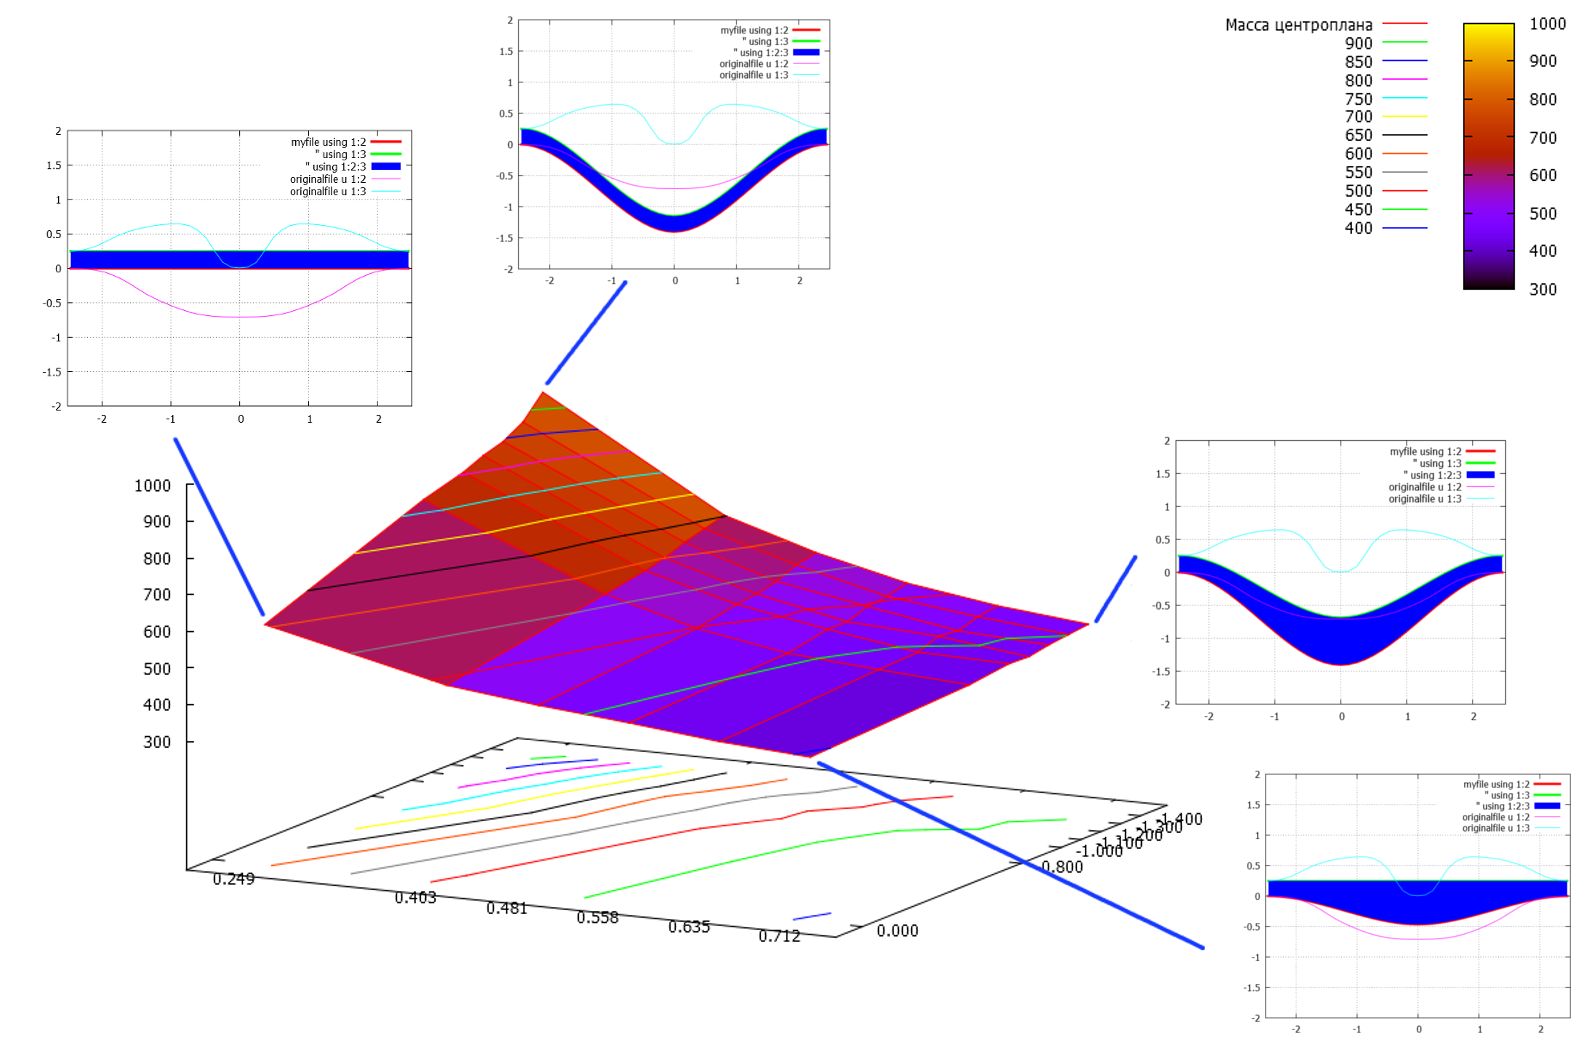
\includegraphics[height=0.9\textwidth]{Optimization3dplot}
\label{fig:Optimization3dplot}
\end{figure}
\end{landscape}


